% Preamble
\documentclass[../main.tex]{subfiles}

% Document
\begin{document}
\chapter{Results and discussion}\label{ch:results}

To measure the performance of all the algorithms introduced previously in the 
practical part, the simulator presented in the previous section was used.  

For these tests, a dataset of 200 different users was generated. At each time 
step of the algorithms, one of these users was randomly selected as the one who 
accessed the website at that moment (this sampling was performed with replacement, 
meaning that the same user could be selected an unlimited number of times).  

In addition, another dataset of 10 different products to be recommended was generated, 
with two products from each of the previously introduced categories.  

Lastly, the simulator was used with these datasets to check whether the recommendations 
of the different algorithms succeeded in making the user click on the suggested product. 
This was carried out over 25,000 time steps with all algorithms running simultaneously, 
i.e., 25,000 website visits were simulated, and it was checked whether the recommendations 
generated by each of the algorithms resulted in the user clicking on the product or not. 
This process was repeated 5 times, and the metrics from these iterations were averaged and 
analyzed.  

Before comparing the algorithms with each other, this same procedure was followed for 
hyperparameter optimization of the different algorithms. In the case of the $\epsilon$-Greedy 
algorithm, values of the parameter $\epsilon$ from 0.01 to 1 were tested. Among all these 
values, $\epsilon = 0.1$ was the value that achieved the best cumulative reward. The results 
of these tests with different values of the $\epsilon$ parameter can be observed in Figure 
\ref{fig:rec_acum_epsilon_greedy}.  

\begin{figure}[H]
\centering
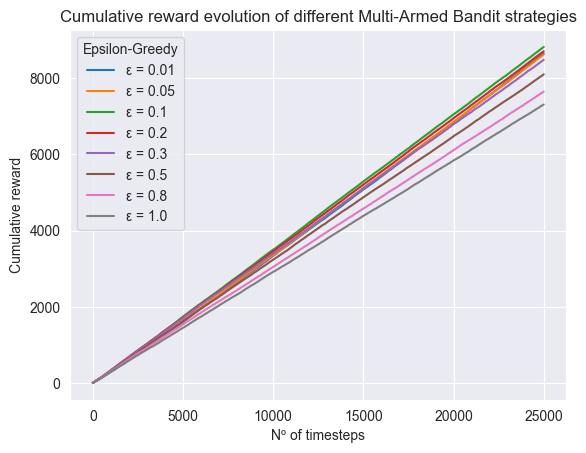
\includegraphics[width=140mm]{../img/rec_acum_epsilon_greedy.png}
\caption{Graph showing the evolution of cumulative reward over time for different values of 
the parameter $\epsilon$ of the $\epsilon$-Greedy algorithm.}
\label{fig:rec_acum_epsilon_greedy}
\end{figure}

For the UCB algorithm, values of the parameter $\alpha$ from 0.05 to 10 were tested, and the 
best results were obtained for $\alpha=0.25$ and $\alpha=0.5$. Between these two values, 
$\alpha=0.25$ was ultimately chosen for use in the comparison between the different algorithms. 
The results of this hyperparameter optimization can be seen in Figure \ref{fig:rec_acum_ucb}.  

\begin{figure}[H]
\centering
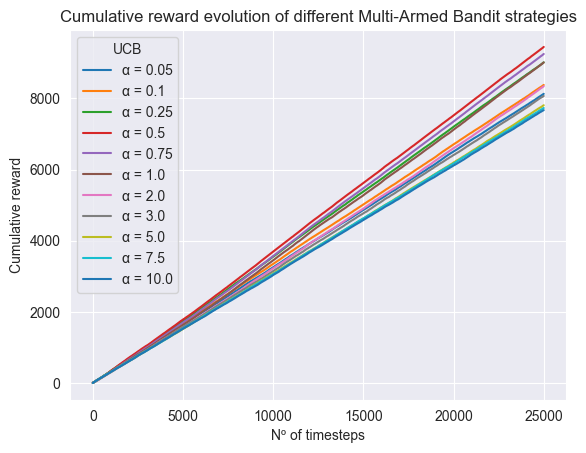
\includegraphics[width=140mm]{../img/rec_acum_ucb.png}
\caption{Graph showing the evolution of cumulative reward over time for different values of 
the parameter $\alpha$ of the UCB algorithm.}
\label{fig:rec_acum_ucb}
\end{figure}

For the LinUCB algorithm, it was found that in this case the values of $\alpha$ that yielded 
the best results were $\alpha = 0.75$ and $\alpha = 1$, among all those tested (the same values 
as for UCB were tested). Between these two values, $\alpha = 0.75$ was chosen for the comparison 
between the different algorithms. The results of these tests can be seen in Figure 
\ref{fig:rec_acum_linucb}.  

\begin{figure}[H]
\centering
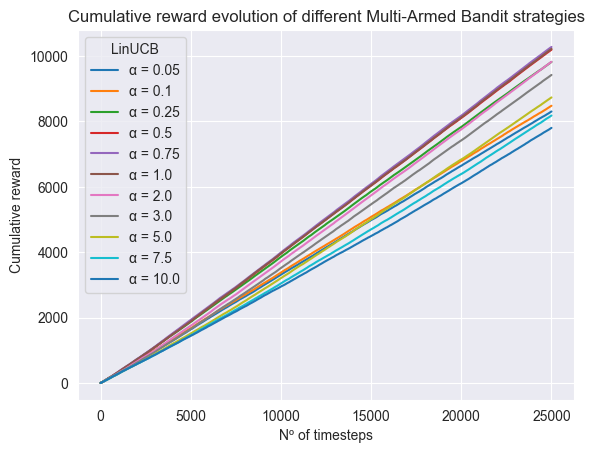
\includegraphics[width=140mm]{../img/rec_acum_linucb.png}
\caption{Graph showing the evolution of cumulative reward over time for different values of the 
parameter $\alpha$ of the LinUCB algorithm.}
\label{fig:rec_acum_linucb}
\end{figure}

And for the LinTS algorithm, values of the parameter $\nu$ between 0.1 and 5 were tested, with 
the best results being obtained for $\nu = 0.3$. These results are shown in Figure 
\ref{fig:rec_acum_lints}.  

\begin{figure}[H]
\centering
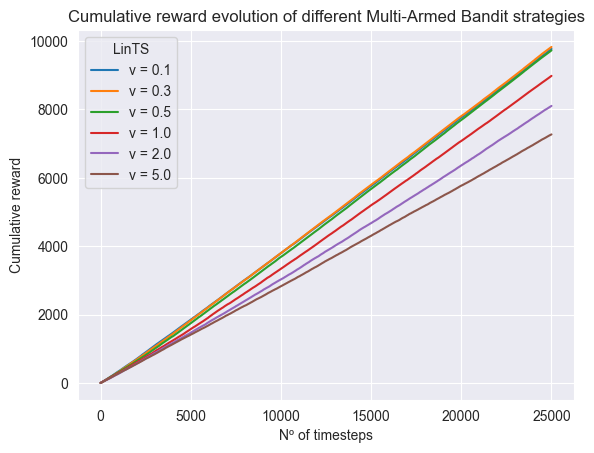
\includegraphics[width=140mm]{../img/rec_acum_lints.png}
\caption{Graph showing the evolution of cumulative reward over time for different values of the 
parameter $\nu$ of the LinTS algorithm.}
\label{fig:rec_acum_lints}
\end{figure}

Once the hyperparameters of all algorithms had been optimized, a comparison between the algorithms 
was carried out. For this purpose, the previously mentioned parameter values were used, and the 
values of the metrics obtained from each of the algorithms were compared.  

Regarding the evolution of cumulative rewards, in the graph shown in Figure \ref{fig:rec_acum_all} 
it can be observed that, as expected, contextual algorithms are superior to those that ignore 
context when such context is available, and all of these algorithms, with or without context, 
clearly outperform selecting products to recommend completely at random. In particular, the LinTS 
algorithm achieves slightly better results than LinUCB, making it the best among all those studied 
for this specific case.  

\begin{figure}[H]
\centering
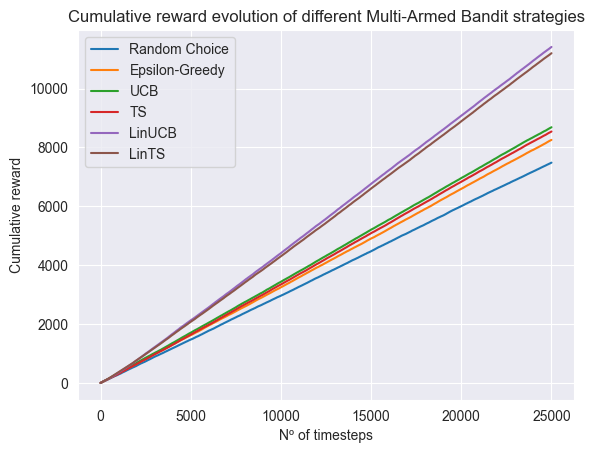
\includegraphics[width=140mm]{../img/rec_acum_all.png}
\caption{Graph showing the evolution of cumulative reward over time for the different 
algorithms used.}
\label{fig:rec_acum_all}
\end{figure}

On the other hand, if the cumulative regret is observed (Figure \ref{fig:reg_acum_all}), the ranking 
from best to worst performance of the algorithms was practically the same (note that in the case of 
cumulative regret, the goal is for it to be as low as possible). The algorithm with the lowest 
cumulative regret was also LinTS, closely followed by LinUCB, and with a clear advantage over the rest 
of the algorithms.  

\begin{figure}[H]
\centering
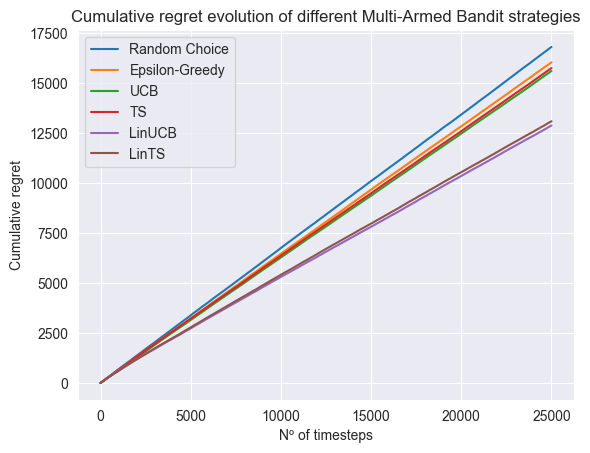
\includegraphics[width=140mm]{../img/reg_acum_all.png}
\caption{Graph showing the evolution of cumulative regret over time for the different algorithms 
used.}
\label{fig:reg_acum_all}
\end{figure}

In addition to these two metrics, the success rate and the accuracy of the algorithms were also 
measured, and the results can be seen in Table \ref{tab:success_precision_table}. For these metrics, 
LinTS was also the algorithm that achieved the best results.  

\begin{table}[H]
\centering
\begin{tabular}{l c c}
\hline
\rowcolor[HTML]{EFEFEF}
\textbf{Algorithm} & \textbf{Success rate} & \textbf{Accuracy} \\
\hline
Random choice & 0,261 & 0,099 \\
\rowcolor[HTML]{E6E6E6}
Epsilon-Greedy & 0,336 & 0,283 \\
UCB & 0,349 & 0,321 \\
\rowcolor[HTML]{E6E6E6}
TS & 0,344 & 0,307 \\
LinUCB & 0,395 & 0,657 \\
\rowcolor[HTML]{E6E6E6}
LinTS & 0,401 & 0,744 \\
\hline
\end{tabular}
\caption{Results of the success rate and accuracy of all the algorithms used.}
\label{tab:success_precision_table}
\end{table}

Regarding cumulative regret, it should be noted that in this case it was 
computed from empirical data using the following formula:  

\begin{equation*}
    R\left(T\right) = \sum_{t=1}^{T}\left(\hat{r}_{t} - r_{t}\right)
\end{equation*}

where $r_{t}$ is the reward of the algorithm selected at that time step and 
$\hat{r}_{t}$ is, among all possible rewards that could have occurred at that 
time step given the recommended product, the highest one.  
 
The use of this alternative formula for computing cumulative regret is due to the 
fact that the theoretical formula introduced previously in the state of the art cannot 
be directly applied in practice in most cases, since in some situations the action with 
optimal reward is unknown, or, as in this case, due to the stochastic nature of the 
process (as it involves sampling from a Bernoulli distribution), the optimal action, 
defined as the one with the highest probability of a successful recommendation, may not 
be successful, while another action with lower probability of success may actually succeed. 
This could lead to regret, when computed using the theoretical formula, becoming negative 
at some time step, which is not possible by definition, as explained in \textcite{loomes1982}.  
\end{document}